\documentclass{article}

\usepackage{amsmath, amsthm, amssymb, amsfonts}
\usepackage{thmtools}
\usepackage{graphicx}
\usepackage{setspace}
\usepackage{geometry}
\usepackage{float}
\usepackage{hyperref}
\usepackage[utf8]{inputenc}
\usepackage[english]{babel}
\usepackage{framed}
\usepackage[dvipsnames]{xcolor}
\usepackage{tcolorbox}

\colorlet{LightGray}{White!90!Periwinkle}
\colorlet{LightOrange}{Orange!15}
\colorlet{LightGreen}{Green!15}

\newcommand{\HRule}[1]{\rule{\linewidth}{#1}}

\declaretheoremstyle[name=Theorem,]{thmsty}
\declaretheorem[style=thmsty,numberwithin=subsection]{theorem}
\tcolorboxenvironment{theorem}{colback=LightGray}

\declaretheoremstyle[name=Proposition,]{prosty}
\declaretheorem[style=prosty,numberlike=theorem]{proposition}
\tcolorboxenvironment{proposition}{colback=LightOrange}

\declaretheoremstyle[name=Principle,]{prcpsty}
\declaretheorem[style=prcpsty,numberlike=theorem]{principle}
\tcolorboxenvironment{principle}{colback=LightGreen}

\setstretch{1.2}
\geometry{
    textheight=9in,
    textwidth=5.5in,
    top=1in,
    headheight=12pt,
    headsep=25pt,
    footskip=30pt
}

% ------------------------------------------------------------------------------

\begin{document}

% ------------------------------------------------------------------------------
% Cover Page and ToC
% ------------------------------------------------------------------------------

\title{ \normalsize \textsc{}
		\\ [2.0cm]
		\HRule{1.5pt} \\
		\LARGE \textbf{\uppercase{Sistema de taquería}
		\HRule{2.0pt} \\ [0.6cm] \LARGE{Unidad 3. Ingeniería de requisitos} \vspace*{8\baselineskip}}
		}
\date{}
\author{\textbf{Presenta:} \\
        \textbf{Josua Nathaniel Arrazola Elizondo} \\
        \textbf{Ricardo Emanuel Uriegas Ibarra} \\
        \textbf{Hector Israel Cruz Resendez} \\
        \textbf{Cristobal Elias Escandon Escobar} \\
        \textbf{Jose Manuel Alonso Cepeda} \\
        \textbf{Alexis Guadalupe Medina Ayala} \\
        \textbf{Rodrigo Santamaria Martinez} \\ \\
		Profesora: Maria Raquel Ortiz Alvarez \\
		Ciudad Victoria, Tamaulipas. \\
		Diciembre 2024}
\maketitle
\newpage

\tableofcontents
% figures
\listoffigures
\newpage

\section{Introducción}
\subsection{Propósito del documento}

El propósito de este documento es describir el diseño y desarrollo del sistema de gestión para una taquería, incluyendo sus requerimientos funcionales y no funcionales, los casos de uso principales, y la arquitectura del sistema. Este documento servirá como guía para el equipo de desarrollo y como referencia para futuras mejoras y mantenimientos del sistema.

\subsection{Alcance del sistema}

El sistema de taquería está diseñado para gestionar de manera eficiente las operaciones diarias de la taquería, incluyendo la gestión de órdenes, inventario, usuarios y roles. El sistema permitirá a cocineros, meseros, cajeros y administradores iniciar sesión y realizar sus tareas según sus roles. Además, incluirá funcionalidades para notificaciones automáticas a los usuarios pertinentes a través de un sistema de alertas. El alcance del sistema abarca desde la autenticación de usuarios hasta la gestión completa de inventario y ventas, optimizando la experiencia del cliente y la eficiencia operativa del negocio.

% ------------------------------------------------------------------------------
\newpage
\section{Requisitos Funcionales}
\subsection{2.1 RF1. Iniciar Sesión}
\begin{itemize}
    \item \textbf{Descripción}: El sistema permitirá a los usuarios autenticarse ingresando sus credenciales.
    \item \textbf{Regla}: Las credenciales ingresadas deben ser verificadas y validadas antes de otorgar acceso. En caso de credenciales incorrectas, se mostrará un mensaje de error.
\end{itemize}

\subsection{2.2 RF2. Gestión de Órdenes}
\begin{itemize}
    \item \textbf{Descripción}: El sistema permitirá gestionar órdenes, incluyendo la creación, modificación, cancelación y consulta de órdenes existentes.
    \item \textbf{Regla}: Solo los usuarios autorizados según su rol podrán realizar acciones sobre las órdenes.
\end{itemize}

\subsection{2.3 RF3. Gestión de Inventario}
\begin{itemize}
    \item \textbf{Descripción}: El sistema permitirá la gestión del inventario de productos, incluyendo la adición, eliminación y modificación de los niveles de inventario.
    \item \textbf{Regla}: Solo los administradores podrán modificar el inventario. Las actualizaciones al inventario deben reflejarse en tiempo real.
\end{itemize}

\subsection{2.4 RF4. Consulta de Inventario}
\begin{itemize}
    \item \textbf{Descripción}: El sistema permitirá a los usuarios consultar el estado actual del inventario para verificar la disponibilidad de productos.
    \item \textbf{Regla}: Todos los usuarios autenticados podrán acceder a la consulta del inventario, pero solo algunos según su rol podrán modificarlo.
\end{itemize}

\subsection{2.5 RF5. Historial de Ventas}
\begin{itemize}
    \item \textbf{Descripción}: El sistema mantendrá un historial de ventas que permitirá la consulta de transacciones anteriores.
    \item \textbf{Regla}: Solo los administradores y cajeros podrán acceder al historial de ventas.
\end{itemize}

\subsection{2.6 RF6. Gestión de Usuarios}
\begin{itemize}
    \item \textbf{Descripción}: El sistema permitirá la administración de usuarios, incluyendo la creación, eliminación y modificación de perfiles de usuario y asignación de roles.
    \item \textbf{Regla}: Solo los administradores podrán gestionar usuarios. Todas las modificaciones deben registrarse en el sistema para auditoría.
\end{itemize}

\subsection{2.7 RF7. Generación de Tickets}
\begin{itemize}
    \item \textbf{Descripción}: El sistema generará tickets para cada orden finalizada, proporcionando un registro impreso de la transacción.
    \item \textbf{Regla}: Los tickets deben contener información detallada de la orden, incluyendo productos, cantidades, precios y tiempo de transacción.
\end{itemize}

\subsection{2.8 RF8. Cobro de Órdenes}
\begin{itemize}
    \item \textbf{Descripción}: El sistema procesará el cobro de las órdenes, manejando transacciones financieras de manera segura.
    \item \textbf{Regla}: Todas las transacciones deben cumplir con los estándares de seguridad financiera y registrar los detalles de cada cobro.
\end{itemize}

\subsection{2.9 RF9. Notificaciones Automáticas}
\begin{itemize}
    \item \textbf{Descripción}: El sistema notificará automáticamente a los usuarios relevantes sobre eventos importantes, como actualizaciones de órdenes o cambios en el inventario.
    \item \textbf{Regla}: Las notificaciones deben enviarse en tiempo real y ser visibles en el área de trabajo del usuario correspondiente.
\end{itemize}

% ------------------------------------------------------------------------------
\newpage
\section{Requisitos No Funcionales}
\subsection{3.1 NF1. Rendimiento}
\begin{itemize}
    \item \textbf{Descripción}: El sistema debe ser capaz de procesar hasta 100 transacciones por minuto sin degradar el rendimiento.
    \item \textbf{Regla}: El tiempo de respuesta para cualquier operación no deberá exceder los 2 segundos bajo cargas máximas.
\end{itemize}

\subsection{3.2 NF2. Seguridad}
\begin{itemize}
    \item \textbf{Descripción}: El sistema debe proteger la información sensible mediante el uso de encriptación y autenticación robusta.
    \item \textbf{Regla}: Todas las comunicaciones deben utilizar protocolos HTTPS y las contraseñas deben almacenarse utilizando algoritmos de hash seguros.
\end{itemize}

\subsection{3.3 NF3. Usabilidad}
\begin{itemize}
    \item \textbf{Descripción}: La interfaz de usuario debe ser intuitiva y fácil de usar para minimizar el tiempo de entrenamiento de los empleados.
    \item \textbf{Regla}: Las tareas comunes deben poder realizarse en no más de tres clics y el diseño debe seguir principios de diseño centrado en el usuario.
\end{itemize}

\subsection{3.4 NF4. Disponibilidad}
\begin{itemize}
    \item \textbf{Descripción}: El sistema debe estar disponible 24/7 con un tiempo de inactividad mínimo.
    \item \textbf{Regla}: La disponibilidad del sistema debe ser del 99.9\%, permitiendo un máximo de 8.76 minutos de inactividad al año.
\end{itemize}

\subsection{3.5 NF5. Mantenibilidad}
\begin{itemize}
    \item \textbf{Descripción}: El sistema debe ser fácil de mantener y actualizar con mínimas interrupciones en el servicio.
    \item \textbf{Regla}: El código debe seguir estándares de codificación claros y estar bien documentado para facilitar las modificaciones futuras.
\end{itemize}

\subsection{3.6 NF6. Escalabilidad}
\begin{itemize}
    \item \textbf{Descripción}: El sistema debe ser escalable para manejar un aumento en el número de usuarios y transacciones sin requerir una reestructuración significativa.
    \item \textbf{Regla}: La arquitectura del sistema debe permitir la adición de recursos de hardware y software de manera modular.
\end{itemize}

\subsection{3.7 NF7. Compatibilidad}
\begin{itemize}
    \item \textbf{Descripción}: El sistema debe ser compatible con los principales navegadores web y sistemas operativos utilizados por los empleados.
    \item \textbf{Regla}: Debe funcionar correctamente en las versiones más recientes de Chrome, Firefox, y Safari, así como en sistemas operativos Linux, Windows y macOS.
\end{itemize}

\subsection{3.8 NF8. Portabilidad}
\begin{itemize}
    \item \textbf{Descripción}: El sistema debe poder ser desplegado en diferentes entornos sin requerir cambios significativos.
    \item \textbf{Regla}: Debe soportar despliegues en servidores locales y en la nube, utilizando contenedores Docker para facilitar la portabilidad.
\end{itemize}

% ------------------------------------------------------------------------------
\newpage
\section{Casos de Uso Principales}
% caso de uso 1: iniciar sesión
\subsection{Caso de uso 1: Iniciar Sesión}

\begin{table}[H]
    \centering
    \begin{tabular}{|l|p{12cm}|}
    \hline
    \textbf{Caso de Uso} & \textbf{Iniciar Sesión} \\ \hline
    \textbf{Actor} & Cocinero, Mesero, Cajero, Administrador \\ \hline
    \textbf{Precondición} & El usuario debe estar registrado en el sistema y sus credenciales deben ser válidas. \\ \hline
    \textbf{Descripción} & Permitir que los usuarios accedan al sistema introduciendo sus datos. Esto asegura que solo los usuarios autorizados puedan interactuar con el sistema según su rol. \\ \hline
    \textbf{Flujo principal} & 
    \begin{enumerate}
        \item El usuario accede a la pantalla de inicio de sesión.
        \item El usuario introduce su nombre de usuario y contraseña.
        \item El sistema verifica que las credenciales coincidan con un usuario que ya esté registrado.
        \item El sistema valida que la cuenta se encuentre activa y no bloqueada.
        \item Si las credenciales son válidas, el sistema muestra el panel principal correspondiente al rol del usuario.
    \end{enumerate} \\ \hline
    \textbf{Excepciones} & 
    \begin{enumerate}
        \item \textbf{Las credenciales no son válidas:} El sistema muestra un mensaje de error indicando que el nombre de usuario o la contraseña son incorrectos.
        \item \textbf{La cuenta está bloqueada:} El sistema informa al usuario que su cuenta no está activa y le proporciona instrucciones para desbloquearla.
    \end{enumerate} \\ \hline
    \textbf{Postcondición} & El usuario accede al sistema con los permisos y funcionalidades correspondientes a su rol. \\ \hline
    \end{tabular}
    \caption{Descripción del Caso de Uso: Iniciar Sesión}
    \label{tab:caso_uso_iniciar_sesion}
\end{table}
    
% caso de uso 2: gestionar ordenes

\subsection{Caso de uso 2: Gestionar Ordenes}

\begin{table}[H]
    \centering
    \begin{tabular}{|l|p{12cm}|}
    \hline
    \textbf{Caso de Uso} & \textbf{Gestionar Órdenes} \\ \hline
    \textbf{Actor} & Mesero, Cajero \\ \hline
    \textbf{Precondición} & El sistema debe estar activo, y el usuario debe haber iniciado sesión con un rol que le permita gestionar órdenes. \\ \hline
    \textbf{Descripción} & Permitir a los meseros y cajeros gestionar las órdenes de los clientes, registrando una nueva, modificándola, eliminándola o consultándola. \\ \hline
    \textbf{Flujo principal} & 
    \begin{enumerate}
        \item El usuario selecciona "Gestionar Órdenes" en el sistema.
        \item El sistema muestra las opciones disponibles: Crear, Modificar, Eliminar o Consultar órdenes.
        \item El usuario elige la acción deseada, pudiendo ser una de las siguientes:
        \begin{itemize}
            \item \textbf{Crear:} El usuario introduce los datos de la nueva orden (mesa, productos, cantidades).
            \item \textbf{Modificar:} El usuario selecciona una orden existente y actualiza los datos necesarios.
            \item \textbf{Eliminar:} El usuario selecciona una orden existente para eliminarla.
            \item \textbf{Consultar:} El usuario selecciona una orden para ver sus detalles.
        \end{itemize}
        \item El sistema guarda los cambios o muestra la información requerida.
    \end{enumerate} \\ \hline
    \textbf{Excepciones} & 
    \begin{enumerate}
        \item \textbf{No se encuentra la orden solicitada:} El sistema muestra un mensaje indicando que no se puede completar la acción.
        \item \textbf{Error al guardar los cambios:} El sistema notifica al usuario y solicita que intente nuevamente.
    \end{enumerate} \\ \hline
    \textbf{Postcondición} & La orden se gestiona exitosamente y los cambios se reflejan en el sistema. \\ \hline
    \end{tabular}
    \caption{Descripción del Caso de Uso: Gestionar Órdenes}
    \label{tab:caso_uso_gestionar_ordenes}
\end{table}


% caso de uso 3: consultar inventario

\subsection{Caso de uso 3: Consultar Inventario}

\begin{table}[H]
    \centering
    \begin{tabular}{|l|p{12cm}|} 
    \hline
    \textbf{Caso de Uso} & \textbf{Consultar Inventario} \\ \hline
    \textbf{Actor} & Cocinero, Administrador \\ \hline
    \textbf{Precondición} & El usuario debe haber iniciado sesión con un rol que tenga permisos para consultar el inventario. \\ \hline
    \textbf{Descripción} & Permitir al usuario visualizar los productos disponibles en el inventario, incluyendo la cantidad de estos en existencia. \\ \hline
    \textbf{Flujo principal} & 
    \begin{enumerate}
        \item El usuario accede a "Consultar Inventario" desde el sistema.
        \item El sistema muestra una lista con los productos disponibles y su cantidad en existencia.
        \item El usuario puede realizar las siguientes acciones:
        \begin{itemize}
            \item Buscar un producto específico utilizando filtros (nombre, categoría).
            \item Ordenar la lista según nombre, cantidad o categoría.
        \end{itemize}
        \item El usuario visualiza los datos requeridos.
    \end{enumerate} \\ \hline
    \textbf{Excepciones} & 
    \begin{enumerate}
        \item \textbf{No hay productos registrados:} El sistema muestra un mensaje indicando que no hay inventario disponible.
    \end{enumerate} \\ \hline
    \textbf{Postcondición} & El usuario obtiene información actualizada del inventario. \\ \hline
    \end{tabular}
    \caption{Descripción del Caso de Uso: Consultar Inventario}
    \label{tab:caso_uso_consultar_inventario}
\end{table}

% caso de uso 4: ver historial de ventas

\subsection{Caso de uso 4: Ver Historial de Ventas}

\begin{table}[H]
    \centering
    \begin{tabular}{|p{3.5cm}|p{10cm}|}
    \hline
    \textbf{Caso de Uso}   & Ver Historial de Ventas (CU6) \\ \hline
    \textbf{Actor}         & Cajero, Administrador \\ \hline
    \textbf{Precondición}  & 
    El actor debe estar autenticado y tener permisos para consultar el historial de ventas. \\ \hline
    \textbf{Descripción}   & 
    Permitir al cajero o administrador consultar el historial de ventas, mostrando información detallada de las transacciones, como el monto total, los productos vendidos y la fecha de la venta. \\ \hline
    \textbf{Flujo Principal} & 
    \begin{enumerate}
        \item El actor accede a la sección \textit{Historial de Ventas}.
        \item El sistema muestra una lista de todas las transacciones realizadas.
        \item El actor selecciona un registro para ver más detalles.
        \item El sistema muestra la información detallada de la venta seleccionada.
        \item El actor puede aplicar filtros de búsqueda (por fecha, monto o producto).
        \item El sistema muestra los resultados filtrados.
    \end{enumerate} \\ \hline
    \textbf{Excepciones}   & 
    \begin{enumerate}
        \item No hay ventas registradas: El sistema muestra un mensaje indicando que no hay registros en el historial.
        \item Error al visualizar los detalles: El sistema informa que hubo un error al intentar mostrar los detalles de la venta.
    \end{enumerate} \\ \hline
    \textbf{Postcondición} & 
    El actor puede ver el historial de ventas y posee acceso a los detalles de cada transacción. \\ \hline
    \end{tabular}
    \caption{Caso de Uso: Ver Historial de Ventas}
    \label{tab:cu6}
\end{table}        
    
% caso de uso 5: gestionar inventario

\subsection{Caso de uso 5: Gestionar Inventario}

\begin{table}[H]
    \centering
    \begin{tabular}{|p{3.5cm}|p{10cm}|}
    \hline
    \textbf{Caso de Uso}   & Gestionar Inventario (CU7) \\ \hline
    \textbf{Actor}         & Administrador \\ \hline
    \textbf{Precondición}  & 
    El actor debe estar autenticado como administrador y tener permisos para gestionar el inventario. \\ \hline
    \textbf{Descripción}   & 
    Permitir al administrador gestionar los productos del inventario, incluyendo agregar nuevos productos, eliminar productos existentes o modificar los detalles de productos ya registrados. \\ \hline
    \textbf{Flujo Principal} & 
    \begin{enumerate}
        \item El administrador accede a la sección \textit{Gestión de Inventario}.
        \item El sistema muestra la lista de productos disponibles en el inventario.
        \item El administrador selecciona una acción: agregar, eliminar o modificar.
        \item Si se selecciona agregar un producto:
        \begin{itemize}
            \item El administrador introduce los datos del producto.
            \item El sistema valida y agrega el producto.
        \end{itemize}
        \item Si se selecciona eliminar un producto:
        \begin{itemize}
            \item El administrador selecciona el producto y confirma la eliminación.
        \end{itemize}
        \item Si se selecciona modificar un producto:
        \begin{itemize}
            \item El administrador selecciona el producto y modifica sus datos.
            \item El sistema guarda los cambios.
        \end{itemize}
    \end{enumerate} \\ \hline    
    \textbf{Excepciones}   & 
    \begin{enumerate}
        \item Los datos del producto son inválidos: El sistema muestra un mensaje de error indicando que los datos proporcionados son incorrectos.
        \item El producto no existe: El sistema muestra un mensaje indicando que el producto no se encuentra en el inventario.
        \item Error al modificar el producto: El sistema muestra un mensaje indicando que no se pudieron guardar los cambios.
    \end{enumerate} \\ \hline
    \textbf{Postcondición} & 
    El inventario se actualiza con las modificaciones realizadas por el administrador. \\ \hline
    \end{tabular}
    \caption{Caso de Uso: Gestionar Inventario (CU7)}
    \label{tab:cu7}
\end{table}

% caso de uso 6: gestionar usuarios

\subsection{Caso de uso 6: Gestionar Usuarios}

\begin{table}[H]
    \centering
    \begin{tabular}{|p{4cm}|p{11cm}|}
    \hline
    \textbf{Caso de Uso}        & \textbf{Gestionar Usuarios} \\ \hline
    \textbf{Actor}              & Administrador \\ \hline
    \textbf{Precondición}       & El administrador debe haber iniciado sesión en el sistema. \\ \hline
    \textbf{Descripción}        & Permitir al administrador gestionar la información de los usuarios, incluyendo acciones como agregar, eliminar o modificar perfiles de usuarios registrados en el sistema. \\ \hline
    \textbf{Flujo Principal}    & 
    \begin{enumerate}
        \item El administrador accede a la sección \textit{Gestión de Usuarios}.
        \item El sistema muestra una lista con los usuarios registrados.
        \item El administrador selecciona una acción: agregar, eliminar o modificar un usuario.
        \item Si se selecciona agregar un usuario:
        \begin{itemize}
            \item El administrador introduce los datos del nuevo usuario (nombre, rol, credenciales).
            \item El sistema valida los datos y crea el usuario.
        \end{itemize}
        \item Si se selecciona eliminar un usuario:
        \begin{itemize}
            \item El administrador selecciona al usuario a eliminar.
            \item El sistema solicita confirmación y elimina el usuario.
        \end{itemize}
        \item Si se selecciona modificar un usuario:
        \begin{itemize}
            \item El administrador selecciona al usuario a modificar.
            \item El sistema permite editar los datos del usuario.
            \item El administrador guarda los cambios y el sistema actualiza el registro.
        \end{itemize}
    \end{enumerate} \\ \hline
    \textbf{Excepciones}        & 
    \begin{enumerate}
        \item Datos inválidos al agregar un usuario: El sistema muestra un mensaje indicando el error y solicita corregirlo.
        \item El administrador intenta eliminar un usuario que no existe: El sistema muestra un mensaje indicando que el usuario no está disponible.
        \item Datos inválidos al modificar un usuario: El sistema notifica los campos inválidos y solicita corregirlos.
    \end{enumerate} \\ \hline
    \textbf{Postcondición}      & Los datos del usuario se gestionan correctamente según la acción realizada (agregar, eliminar o modificar). \\ \hline
    \end{tabular}
    \caption{Caso de Uso: Gestionar Usuarios}
    \label{tab:gestionar_usuarios}
\end{table}

% caso de uso 7: finalizar orden

\subsection{Caso de uso 7: Finalizar Orden}

\begin{table}[H]
    \centering
    \begin{tabular}{|p{3.5cm}|p{10cm}|}
    \hline
    \textbf{Caso de Uso}   & Finalizar Orden (CU12) \\ \hline
    \textbf{Actor}         & Cajero \\ \hline
    \textbf{Precondición}  & 
    Debe existir al menos una orden activa en el sistema. \\ \hline
    \textbf{Descripción}   & 
    Permitir al cajero cerrar una orden activa, registrar el pago, generar un ticket con el desglose del consumo y marcar la orden como finalizada en el sistema. \\ \hline
    \textbf{Flujo Principal} & 
    \begin{enumerate}
        \item El cajero accede a la sección \textit{Finalizar Orden}.
        \item El sistema muestra las órdenes activas.
        \item El cajero selecciona una orden y verifica sus detalles.
        \item El cliente realiza el pago, y el cajero lo registra.
        \item El sistema genera un ticket, actualiza el estado de la orden y almacena el registro en el historial de ventas.
        \item El cajero entrega el ticket al cliente.
    \end{enumerate} \\ \hline
    \textbf{Excepciones}   & 
    \begin{enumerate}
        \item La orden no existe o ya fue finalizada: El sistema informa al cajero.
        \item El pago es insuficiente: El sistema solicita un monto válido.
        \item Error al generar el ticket: El sistema notifica el problema y sugiere reintentar.
    \end{enumerate} \\ \hline
    \textbf{Postcondición} & 
    La orden se registra como finalizada, el ticket se entrega al cliente y el pago se guarda en el historial de ventas. \\ \hline
    \end{tabular}
    \caption{Caso de Uso: Finalizar Orden (CU12)}
    \label{tab:cu12}
\end{table}

% caso de uso 8: notificar al cocinero

\subsection{Caso de uso 8: Notificar al Mesero}

\begin{table}[H]
    \centering
    \begin{tabular}{|p{4cm}|p{11cm}|}
    \hline
    \textbf{Caso de Uso}        & \textbf{Notificar al Cocinero} \\ \hline
    \textbf{Actor}              & Sistema de Alertas \\ \hline
    \textbf{Precondición}       & Una orden debe estar registrada y en estado "pendiente" o "en preparación". \\ \hline
    \textbf{Descripción}        & El sistema envía una notificación al cocinero cuando se registra una nueva orden o se actualiza una orden existente que requiere acción inmediata en la cocina. \\ \hline
    \textbf{Flujo Principal}    & 
    \begin{enumerate}
        \item El mesero o cajero registra o actualiza una orden en el sistema.
        \item El sistema verifica el estado de la orden:
        \begin{itemize}
            \item Si la orden está en estado "pendiente" o "en preparación", procede a notificar.
        \end{itemize}
        \item El sistema genera una notificación para el cocinero con la información de la orden:
        \begin{itemize}
            \item Detalles de la orden (número, productos, cantidades).
            \item Tiempo estimado de preparación.
        \end{itemize}
        \item El cocinero recibe la notificación en la pantalla de la cocina o dispositivo designado.
    \end{enumerate} \\ \hline
    \textbf{Excepciones}        & 
    \begin{enumerate}
        \item No hay conexión con el dispositivo del cocinero: El sistema guarda la notificación en cola y muestra un mensaje al administrador para verificar la conexión.
        \item La información de la orden está incompleta: El sistema envía una alerta al mesero o cajero para corregirla antes de proceder.
    \end{enumerate} \\ \hline
    \textbf{Postcondición}      & El cocinero recibe la notificación con los detalles de la orden para iniciar o continuar su preparación. \\ \hline
    \end{tabular}
    \caption{Caso de Uso: Notificar al Cocinero}
    \label{tab:notificar_cocinero}
\end{table}
    
% caso de uso 9: notificar al mesero

\subsection{Caso de uso 9: Notificar al Mesero}

\begin{table}[H]
    \centering
    \begin{tabular}{|p{4cm}|p{11cm}|}
    \hline
    \textbf{Caso de Uso}        & \textbf{Notificar al Mesero} \\ \hline
    \textbf{Actor}              & Sistema de Alertas \\ \hline
    \textbf{Precondición}       & La orden asignada al mesero debe estar en estado "lista para entregar". \\ \hline
    \textbf{Descripción}        & El sistema notifica al mesero que una orden está lista para ser entregada al cliente, indicando los detalles necesarios para su identificación. \\ \hline
    \textbf{Flujo Principal}    & 
    \begin{enumerate}
        \item El cocinero marca una orden como "lista para entregar" en el sistema.
        \item El sistema identifica al mesero asociado a la orden.
        \item El sistema genera una notificación para el mesero con los siguientes detalles:
        \begin{itemize}
            \item Número de la orden.
            \item Mesa o cliente asociado.
            \item Productos de la orden.
        \end{itemize}
        \item El mesero recibe la notificación en su dispositivo o pantalla asignada.
    \end{enumerate} \\ \hline
    \textbf{Excepciones}        & 
    \begin{enumerate}
        \item No hay un mesero asignado a la orden: El sistema muestra una alerta al administrador para que asigne uno.
        \item La orden no contiene información suficiente para identificarla: El sistema informa al cocinero para corregir los detalles antes de notificar al mesero.
    \end{enumerate} \\ \hline
    \textbf{Postcondición}      & El mesero recibe la notificación y procede con la entrega de la orden al cliente. \\ \hline
    \end{tabular}
    \caption{Caso de Uso: Notificar al Mesero}
    \label{tab:notificar_mesero}
\end{table}

% caso de uso 10: modificar orden

\subsection{Caso de uso 10: Modificar Orden}

\begin{table}[H]
    \centering
    \begin{tabular}{|p{4cm}|p{11cm}|}
    \hline
    \textbf{Caso de Uso}        & \textbf{Modificar Orden} \\ \hline
    \textbf{Actor}              & Mesero \\ \hline
    \textbf{Precondición}       & Debe existir una orden previamente creada y activa en el sistema. \\ \hline
    \textbf{Descripción}        & El mesero realiza cambios en una orden existente, como agregar, eliminar o modificar productos, antes de que sea procesada por el cocinero. \\ \hline
    \textbf{Flujo Principal}    & 
    \begin{enumerate}
        \item El mesero accede al sistema y selecciona la opción \textit{Modificar Orden}.
        \item El sistema muestra una lista de las órdenes activas y el mesero elige una para modificar.
        \item El sistema presenta los detalles de la orden seleccionada.
        \item El mesero realiza las siguientes acciones según sea necesario:
        \begin{itemize}
            \item Agregar productos: selecciona el producto, indica la cantidad, y lo agrega a la orden.
            \item Eliminar productos: selecciona un producto y lo elimina de la orden.
            \item Modificar productos: selecciona un producto, ajusta la cantidad o características, y actualiza la orden.
        \end{itemize}
        \item El mesero guarda los cambios y el sistema actualiza la orden.
    \end{enumerate} \\ \hline
    \textbf{Excepciones}        & 
    \begin{enumerate}
        \item La orden seleccionada no está activa: El sistema informa al mesero que no se pueden realizar cambios.
        \item Se intenta agregar un producto no disponible en inventario: El sistema muestra un mensaje de error indicando que no hay suficiente stock para completar la acción.
    \end{enumerate} \\ \hline
    \textbf{Postcondición}      & La orden queda actualizada con los cambios realizados y lista para ser procesada por el cocinero. \\ \hline
    \end{tabular}
    \caption{Caso de Uso: Modificar Orden}
    \label{tab:modificar_orden}
\end{table}    

% caso de uso 11: Solicitar Modificación de Orden
\subsection{Caso de uso 11: Solicitar Modificación de Orden}

\begin{table}[H]
    \centering
    \begin{tabular}{|p{4cm}|p{11cm}|}
    \hline
    \textbf{Caso de Uso}        & \textbf{Solicitar Modificación de Orden (en caso de error en cobro)} \\ \hline
    \textbf{Actor}              & Cajero \\ \hline
    \textbf{Precondición}       & Debe existir una orden previamente creada y en estado de cobro en el sistema. \\ \hline
    \textbf{Descripción}        & El cajero solicita la modificación de una orden existente debido a un error detectado durante el proceso de cobro. \\ \hline
    \textbf{Flujo Principal}    & 
    \begin{enumerate}
        \item El cajero detecta un error en el cobro de la orden.
        \item El cajero selecciona la opción \textit{Solicitar Modificación de Orden} en el sistema.
        \item El sistema muestra la orden afectada y solicita detalles de la modificación.
        \item El cajero ingresa la modificación requerida y envía la solicitud.
        \item El sistema notifica al Administrador sobre la solicitud de modificación.
        \item El Administrador revisa y aprueba o rechaza la modificación.
        \item Si es aprobado, el sistema actualiza la orden y ajusta el cobro.
        \item El cajero verifica que la modificación ha sido aplicada correctamente.
    \end{enumerate} \\ \hline
    \textbf{Excepciones}        & 
    \begin{enumerate}
        \item El Administrador rechaza la solicitud de modificación: El cajero recibe una notificación de rechazo y no se realiza ninguna modificación.
        \item La orden ya ha sido procesada por cocina: El sistema impide realizar la modificación y notifica al cajero.
    \end{enumerate} \\ \hline
    \textbf{Postcondición}      & La orden ha sido corregida y el cobro se ha ajustado según la modificación aprobada. \\ \hline
    \end{tabular}
    \caption{Caso de Uso: Solicitar Modificación de Orden (en caso de error en cobro)}
    \label{tab:solicitar_modificacion_orden}
\end{table}

\subsection{Caso de Uso 12: Gestionar Roles}

\begin{table}[H]
    \centering
    \begin{tabular}{|p{4cm}|p{11cm}|}
    \hline
    \textbf{Caso de Uso}        & \textbf{Gestionar Roles} \\ \hline
    \textbf{Actor}              & Administrador \\ \hline
    \textbf{Precondición}       & El administrador debe estar autenticado en el sistema con permisos para gestionar roles. \\ \hline
    \textbf{Descripción}        & El administrador asigna, modifica o revoca roles a los usuarios existentes para gestionar sus permisos y acceso a las funcionalidades del sistema. \\ \hline
    \textbf{Flujo Principal}    & 
    \begin{enumerate}
        \item El administrador accede al módulo de gestión de usuarios en el sistema.
        \item El sistema muestra una lista de usuarios actuales.
        \item El administrador selecciona un usuario para gestionar sus roles.
        \item El sistema presenta las opciones de roles disponibles.
        \item El administrador asigna uno o más roles al usuario, modifica los roles existentes o revoca roles según sea necesario.
        \item El administrador guarda los cambios realizados.
        \item El sistema actualiza los permisos del usuario en función de los nuevos roles asignados.
        \item El administrador confirma que los cambios han sido aplicados correctamente.
    \end{enumerate} \\ \hline
    \textbf{Excepciones}        & 
    \begin{enumerate}
        \item El administrador intenta asignar un rol inexistente: El sistema muestra un mensaje de error indicando que el rol no está disponible.
        \item El administrador no tiene permisos suficientes para gestionar roles: El sistema deniega la acción y notifica al administrador.
        \item Fallo en la actualización de roles debido a un error del sistema: El sistema revierte los cambios y notifica al administrador sobre el fallo.
    \end{enumerate} \\ \hline
    \textbf{Postcondición}      & Los roles del usuario han sido actualizados según las modificaciones realizadas por el administrador, reflejando los nuevos permisos y accesos en el sistema. \\ \hline
    \end{tabular}
    \caption{Caso de Uso: Gestionar Roles}
    \label{tab:gestionar_roles}
\end{table}

% ------------------------------------------------------------------------------
\newpage
\section{Riesgos Identificados}

\subsection{R1: Pérdida de Datos}
\begin{itemize}
    \item \textbf{Descripción}: Posibilidad de pérdida de datos por fallos en el sistema o errores humanos.
    \item \textbf{Mitigación}: Realizar backups periódicos y contar con sistemas de recuperación de información.
\end{itemize}

\subsection{R2: Fallos en la Infraestructura Tecnológica}
\begin{itemize}
    \item \textbf{Descripción}: Interrupciones en la infraestructura tecnológica que pueden afectar la operatividad del sistema.
    \item \textbf{Mitigación}: Implementar redundancia en los servidores y realizar mantenimientos preventivos regularmente.
\end{itemize}

\subsection{R3: Brechas de Seguridad}
\begin{itemize}
    \item \textbf{Descripción}: Riesgo de accesos no autorizados a información sensible debido a vulnerabilidades en el sistema.
    \item \textbf{Mitigación}: Utilizar encriptación de datos, implementar autenticación multifactor y realizar auditorías de seguridad periódicas.
\end{itemize}

\subsection{R4: Resistencia al Cambio}
\begin{itemize}
    \item \textbf{Descripción}: Dificultad en la adopción del nuevo sistema por parte de los empleados, lo que puede reducir la eficiencia operativa.
    \item \textbf{Mitigación}: Proporcionar capacitación adecuada, involucrar a los empleados en el proceso de implementación y ofrecer incentivos para el uso del sistema.
\end{itemize}

\subsection{R5: Dependencia de Proveedores Externos}
\begin{itemize}
    \item \textbf{Descripción}: Retrasos o fallos en servicios de terceros que pueden impactar el funcionamiento del sistema.
    \item \textbf{Mitigación}: Diversificar proveedores, establecer acuerdos de nivel de servicio (SLA) claros y mantener planes de contingencia.
\end{itemize}

% ------------------------------------------------------------------------------
\newpage
\section{Aprobación del Documento}
Este documento ha sido revisado y validado con los bibliotecarios. Con la aprobación de está versión, se
procederá al desarrollo del sistema de taqueria.

\begin{table}[h!]
\centering
\begin{tabular}{|p{4cm}|p{5cm}|p{5cm}|}
\hline
\textbf{Rol} & \textbf{Nombre} & \textbf{Firma} \\ \hline
Autor & Jose Manuel Alonso Cepeda & \\ \hline
Coautor & Alexis Guadalupe Medina Ayala & \\ \hline
Coautor & Rodrigo Santamaria Martinez & \\ \hline
Revisor & Maria Raquel Ortiz Alvarez & \\ \hline
\end{tabular}
\caption{Aprobación del Documento}
\label{tab:aprobacion_documento}
\end{table}

\newpage
\section{Conclusión}
Este documento refleja los requisitos funcionales y no funcionales para el sistema de gestión de una taquería. La implementación de este sistema permitirá optimizar la gestión de órdenes, inventario y usuarios, mejorando la experiencia tanto de los empleados como de los clientes de la taquería.

\section{Anexos}
\subsection{Prototipo de la Interfaz}
\begin{figure}[H]
    \centering
    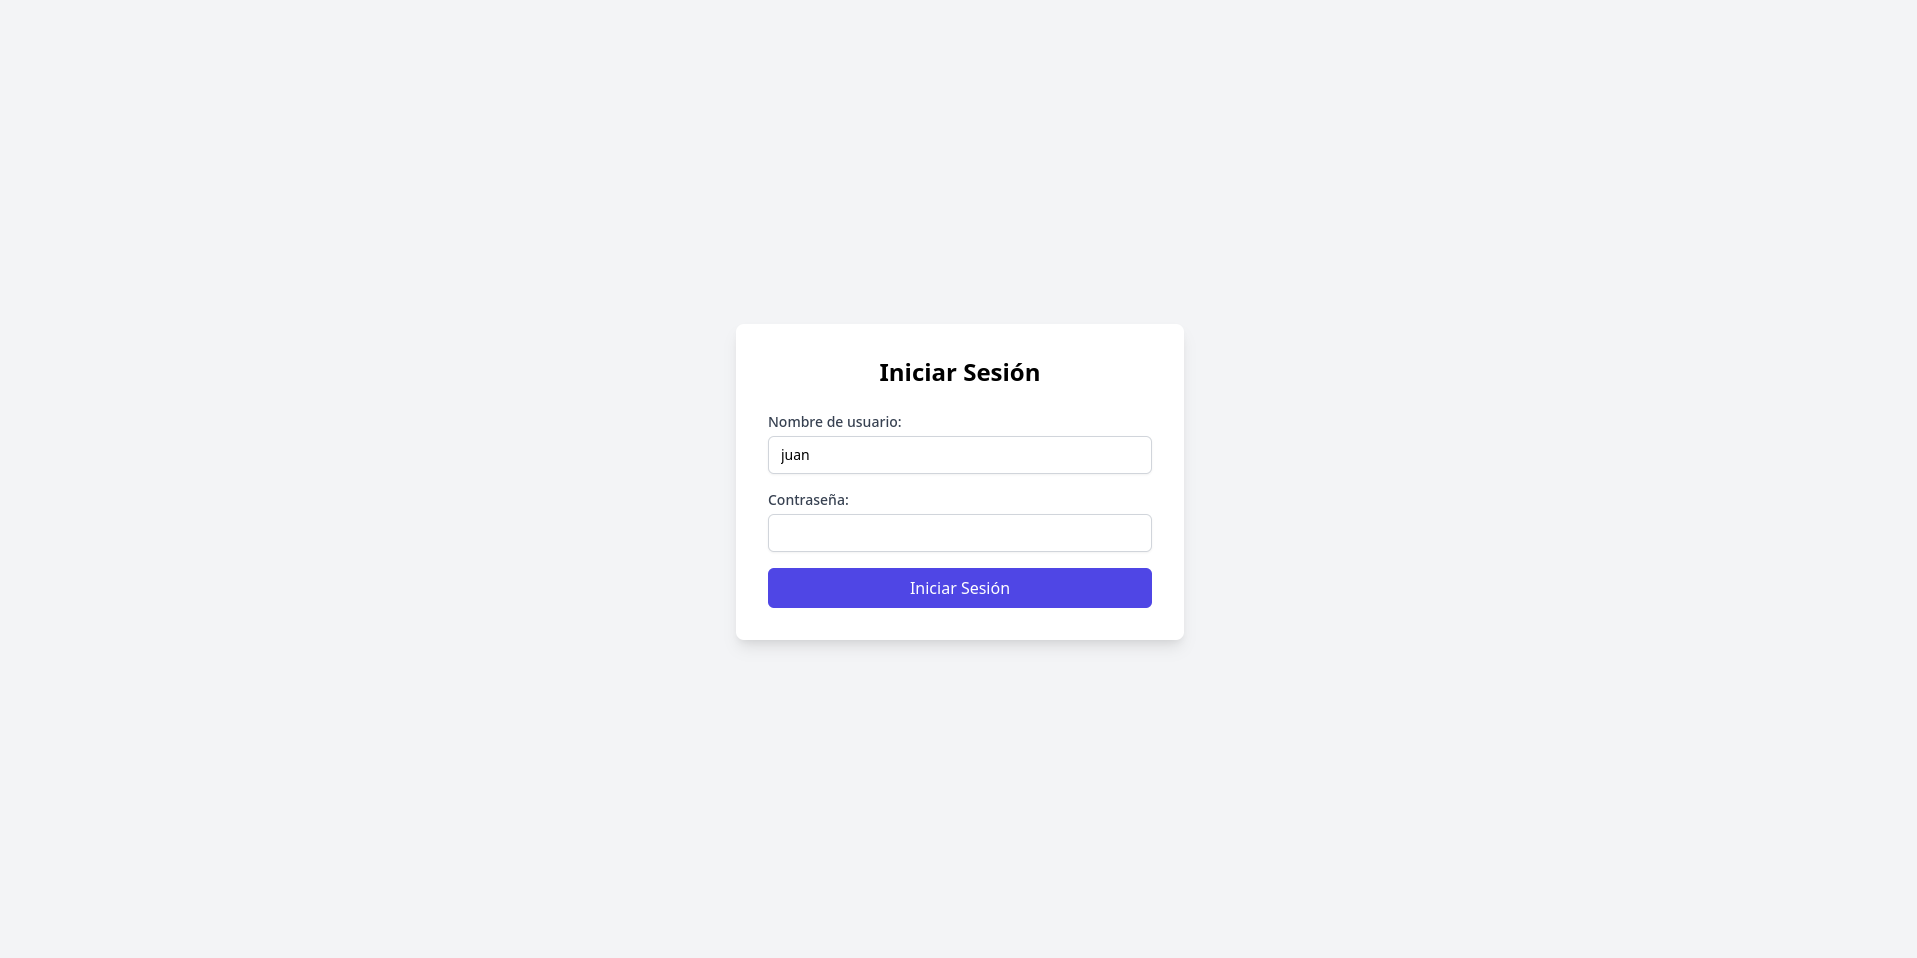
\includegraphics[width=1\textwidth]{img/login.png}
    \caption{Prototipo de la Interfaz del Login del Sistema de Taquería}
    \label{fig:prototipo_interfaz}
\end{figure}

\begin{figure}[H]
    \centering
    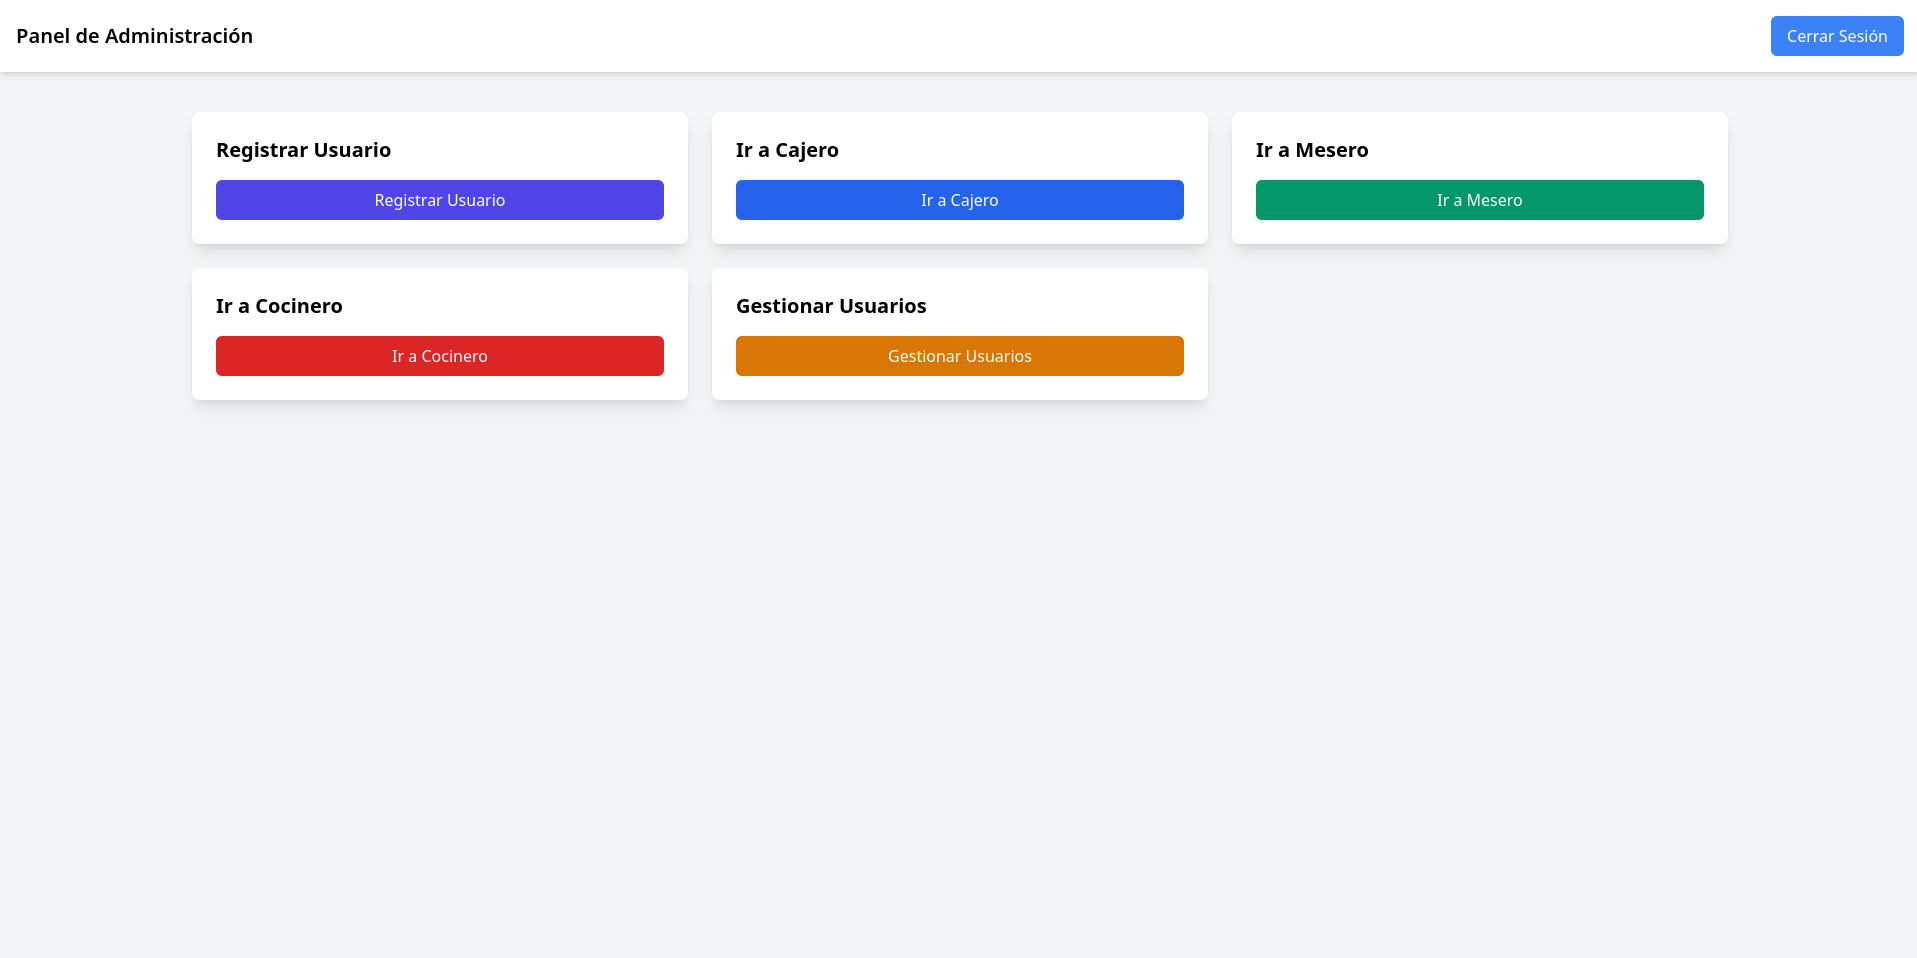
\includegraphics[width=1\textwidth]{img/principal.png}
    \caption{Prototipo de la Interfaz de la Página Principal del Sistema de Taquería observada por un Administrador}
    \label{fig:prototipo_interfaz_ordenes}
\end{figure}

\begin{figure}[H]
    \centering
    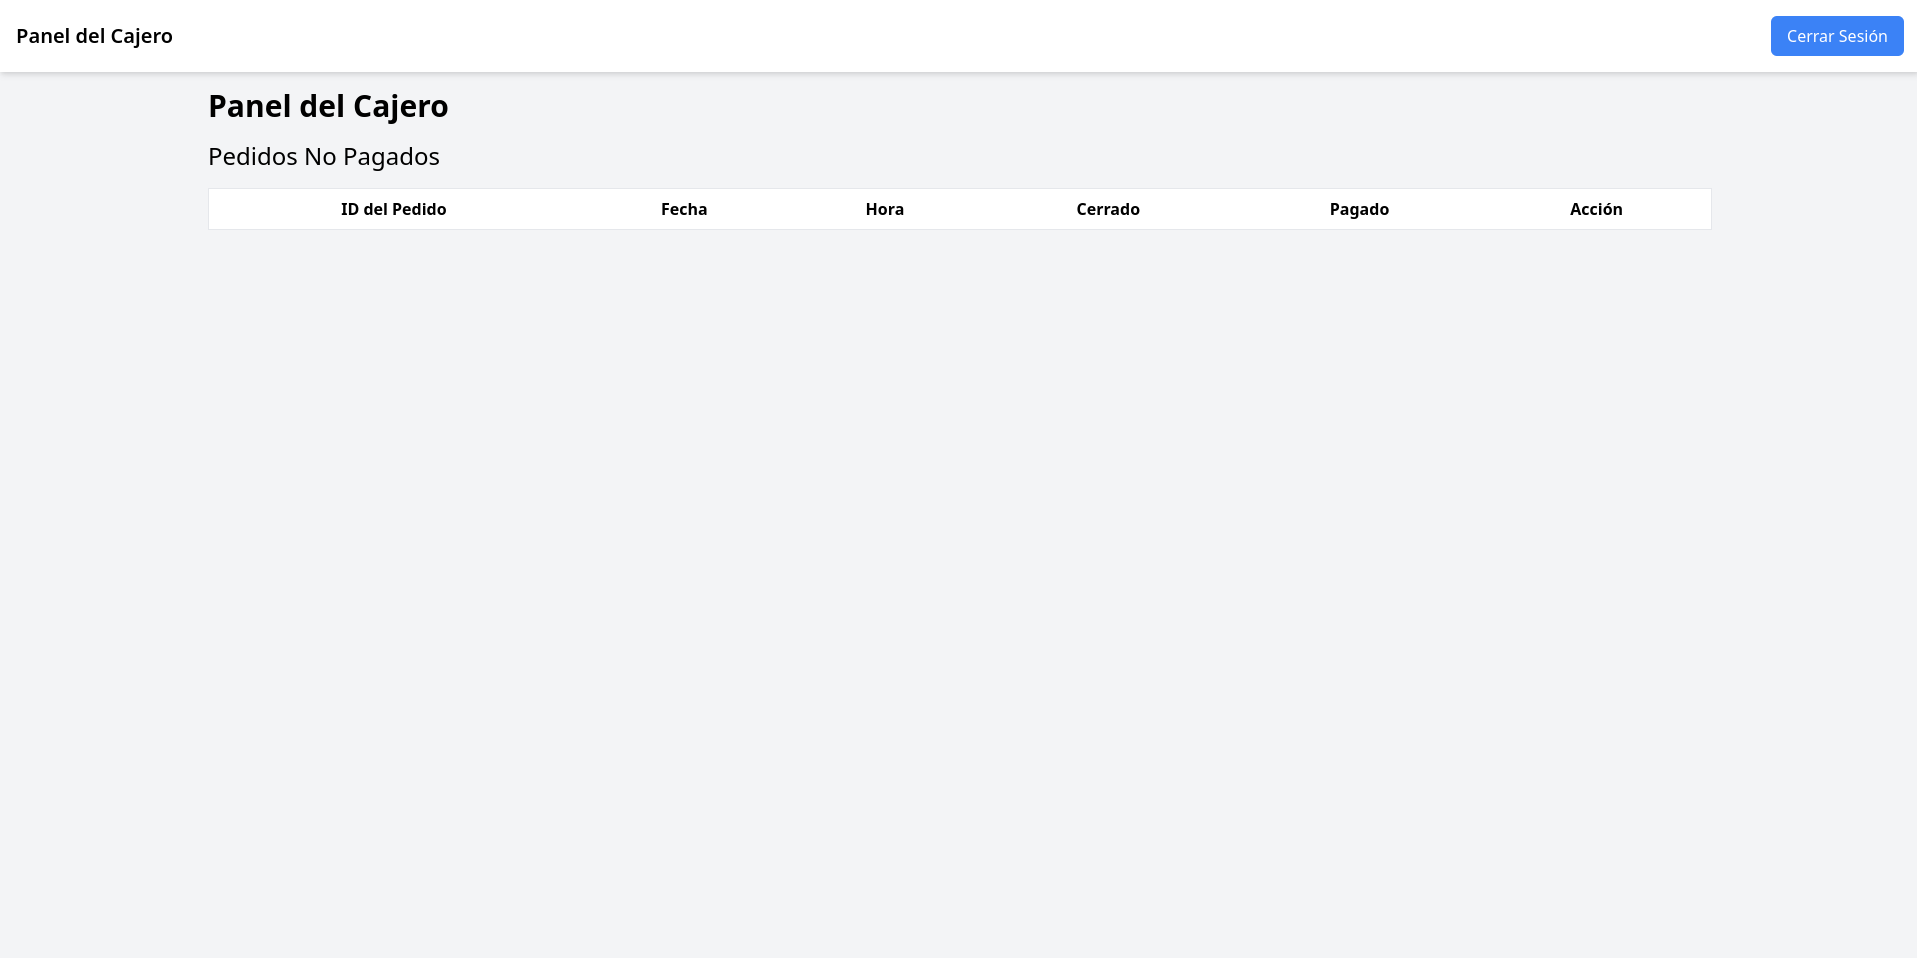
\includegraphics[width=1\textwidth]{img/cajero.png}
    \caption{Prototipo de la Interfaz de la Página Principal del Sistema de Taquería observada por un Cajero}
    \label{fig:prototipo_interfaz_cajero}
\end{figure}

\begin{figure}[H]
    \centering
    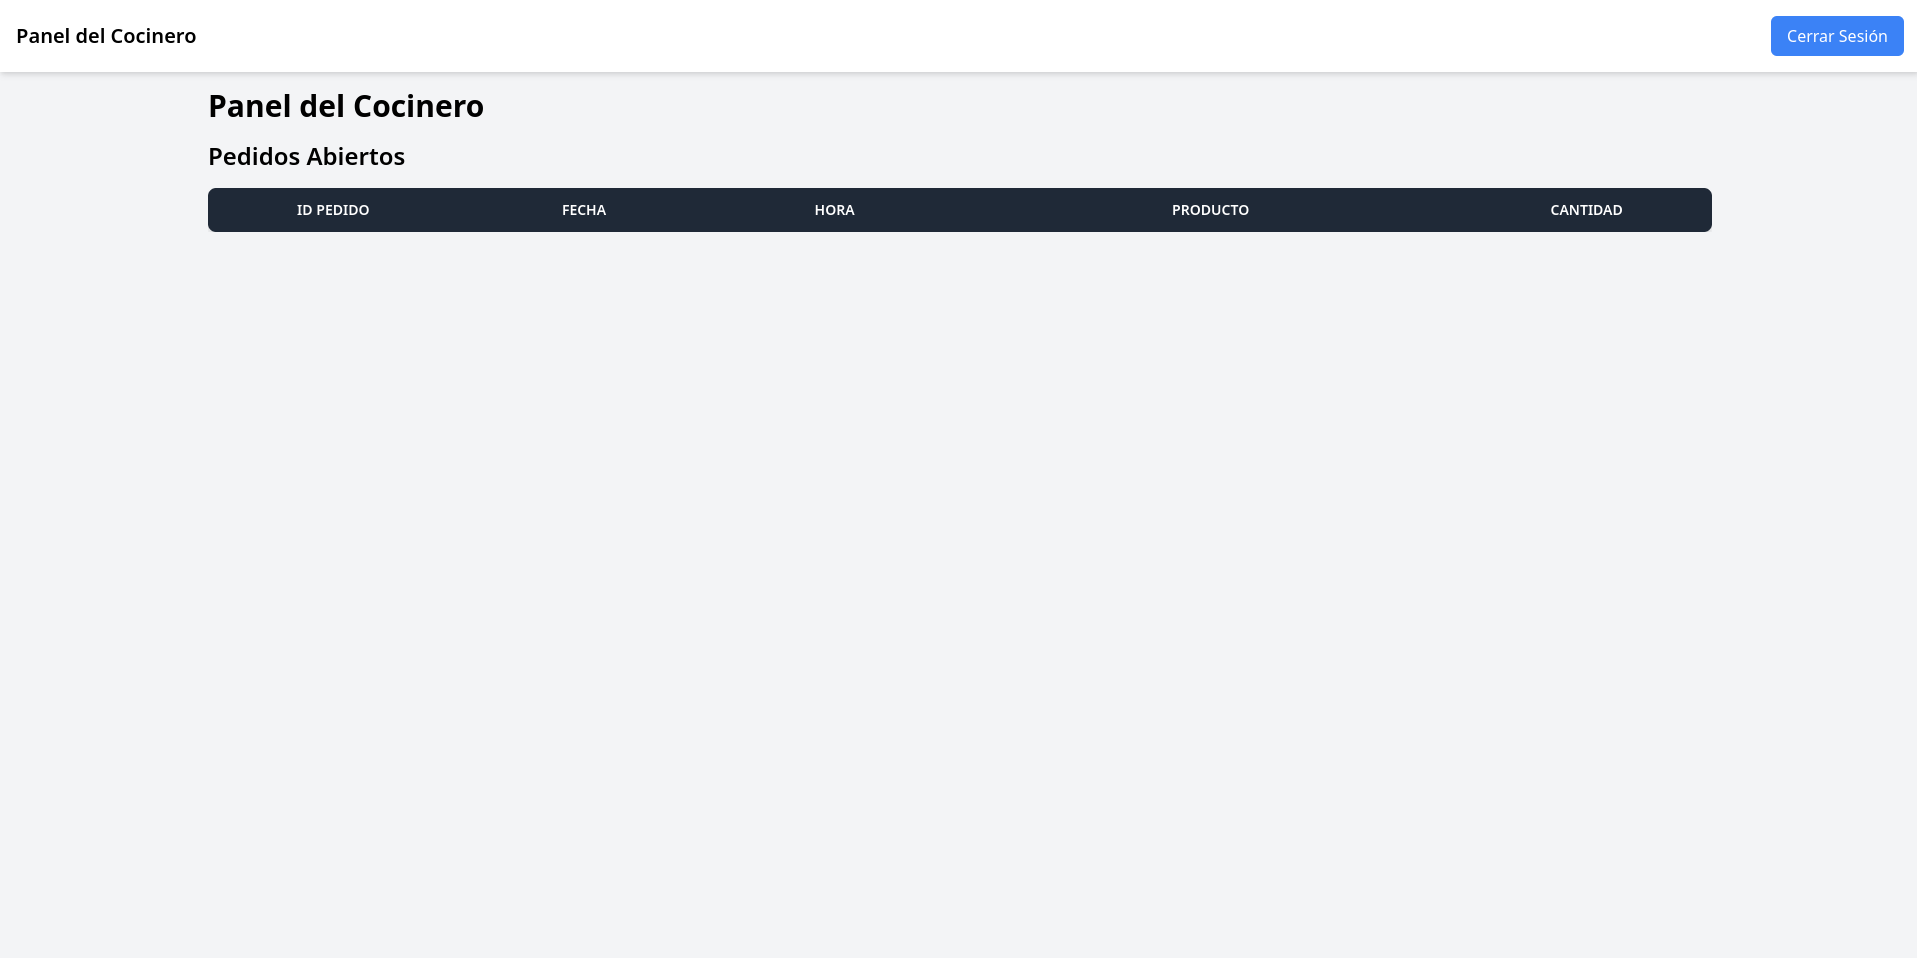
\includegraphics[width=1\textwidth]{img/cocinero.png}
    \caption{Prototipo de la Interfaz de la Página Principal del Sistema de Taquería observada por un Cocinero}
    \label{fig:prototipo_interfaz_cocinero}
\end{figure}

\begin{figure}[H]
    \centering
    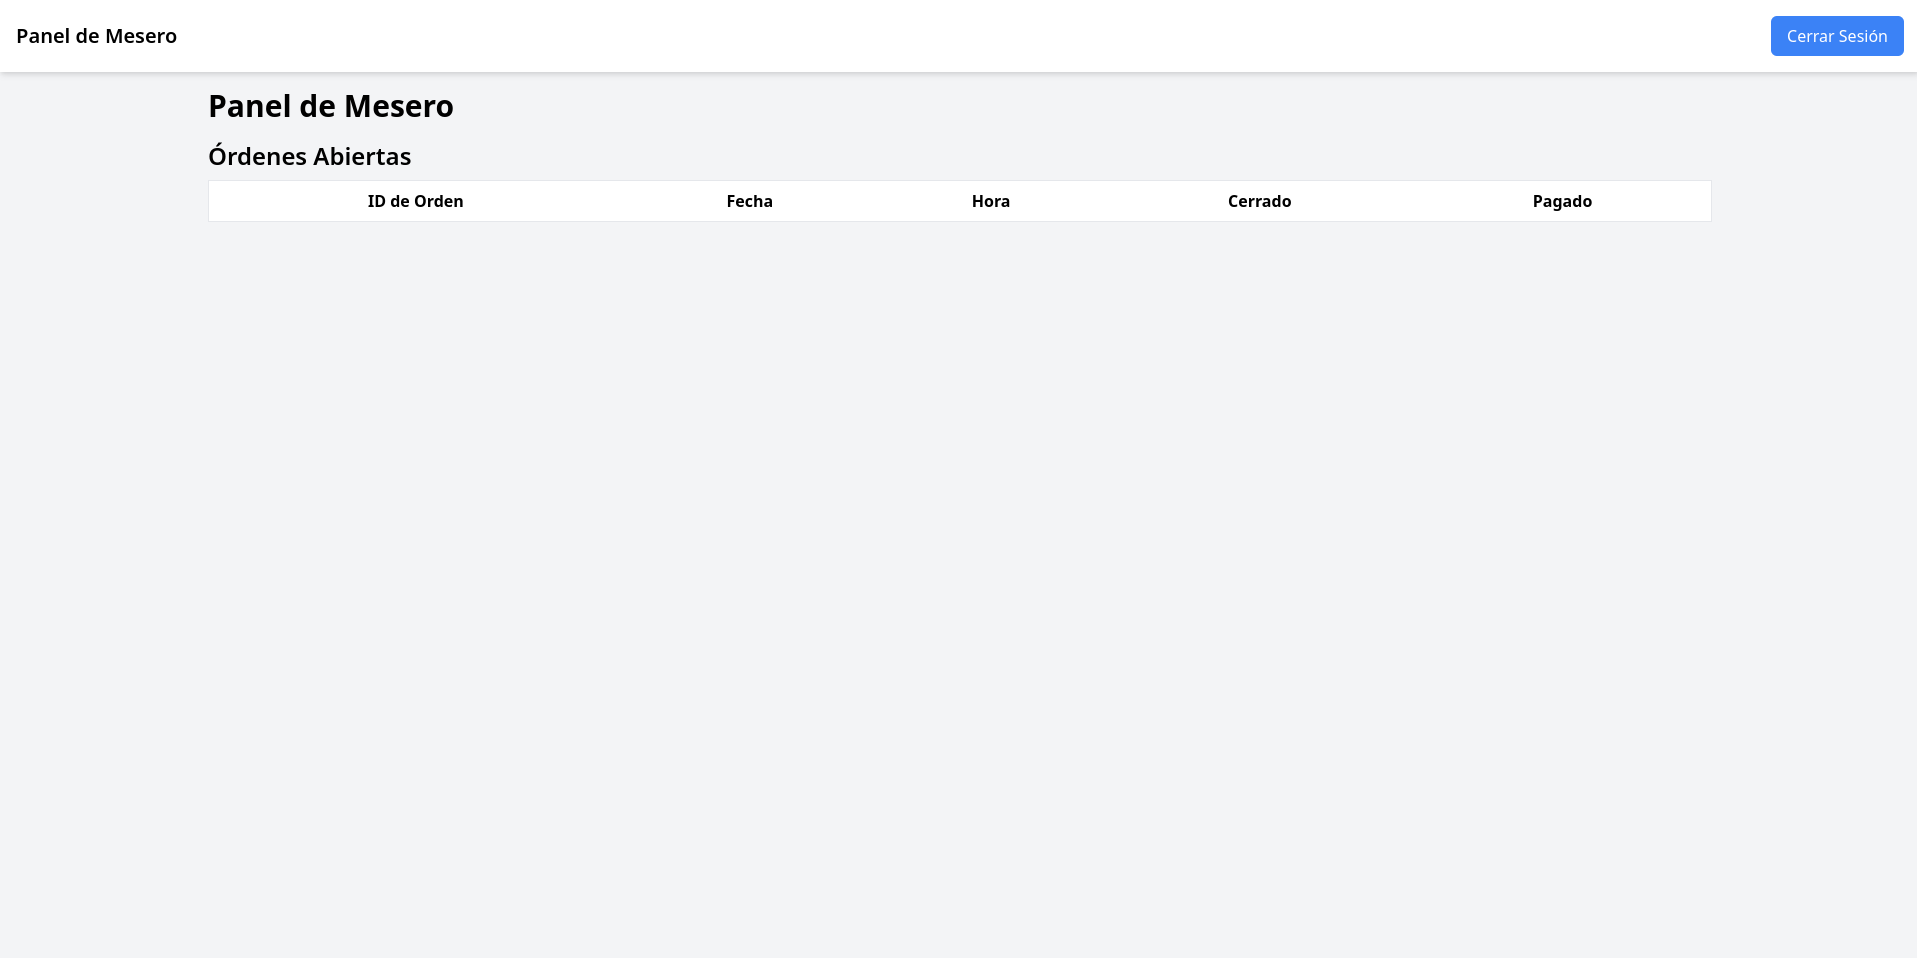
\includegraphics[width=1\textwidth]{img/mesero.png}
    \caption{Prototipo de la Interfaz de la Página Principal del Sistema de Taquería observada por un Mesero}
    \label{fig:prototipo_interfaz_mesero}
\end{figure}

\begin{figure}[H]
    \centering
    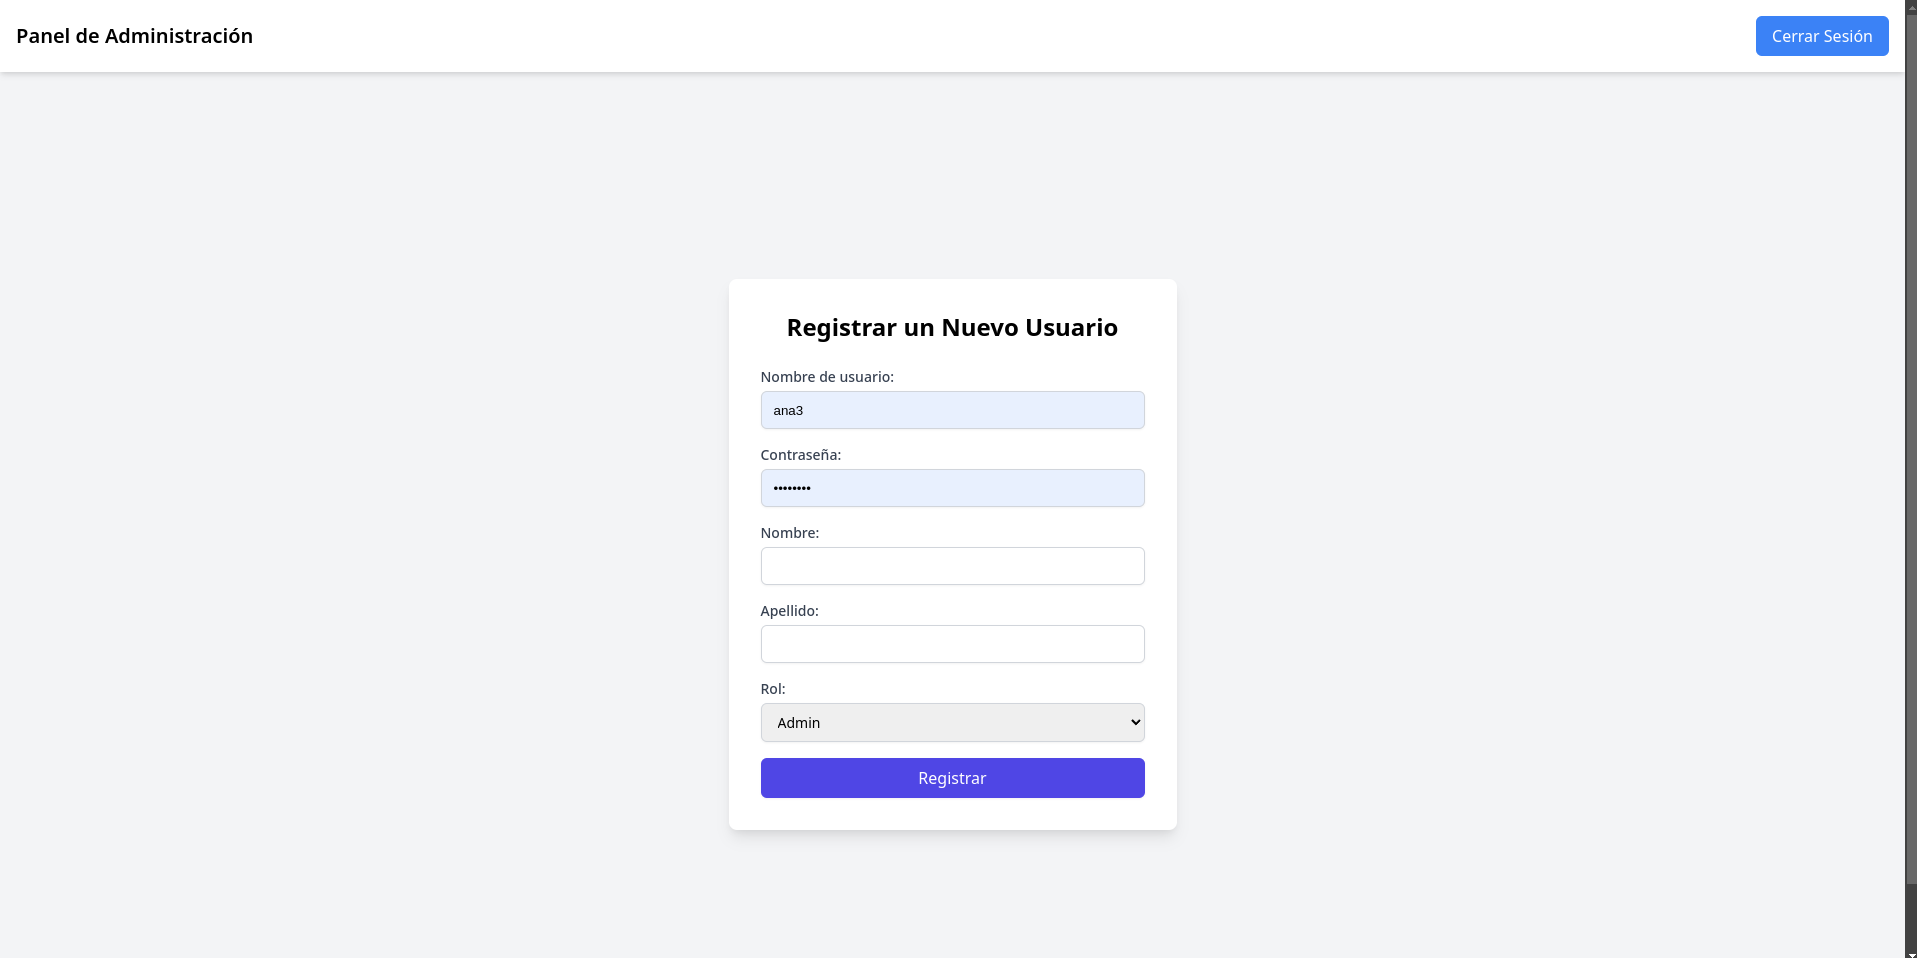
\includegraphics[width=1\textwidth]{img/registrar.png}
    \caption{Prototipo de la Interfaz de la Página para Registrar un nuevo usuario}
    \label{fig:prototipo_interfaz_registrar}
\end{figure}

\begin{figure}[H]
    \centering
    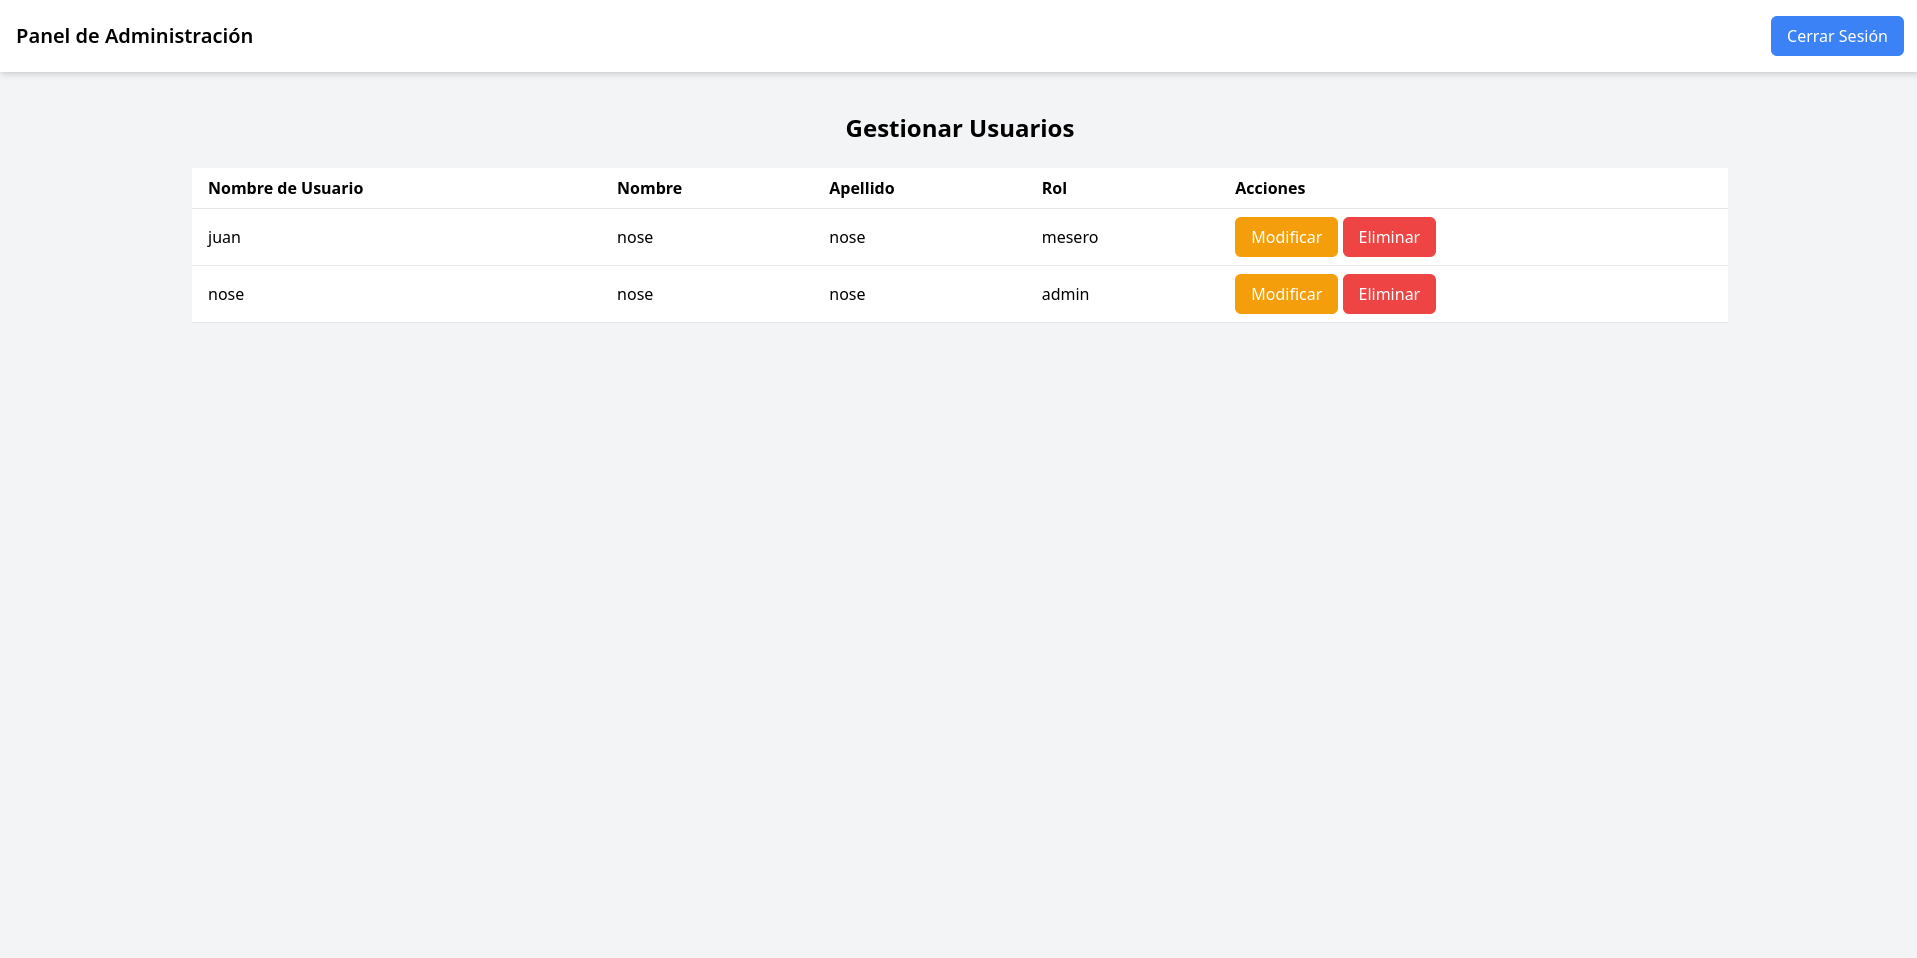
\includegraphics[width=1\textwidth]{img/usuarios.png}
    \caption{Prototipo de la Interfaz de la Página para Gestionar Usuarios}
    \label{fig:prototipo_interfaz_usuarios}
\end{figure}


\subsection{Diagrama de Casos de Uso}
\begin{figure}[H]
    \centering
    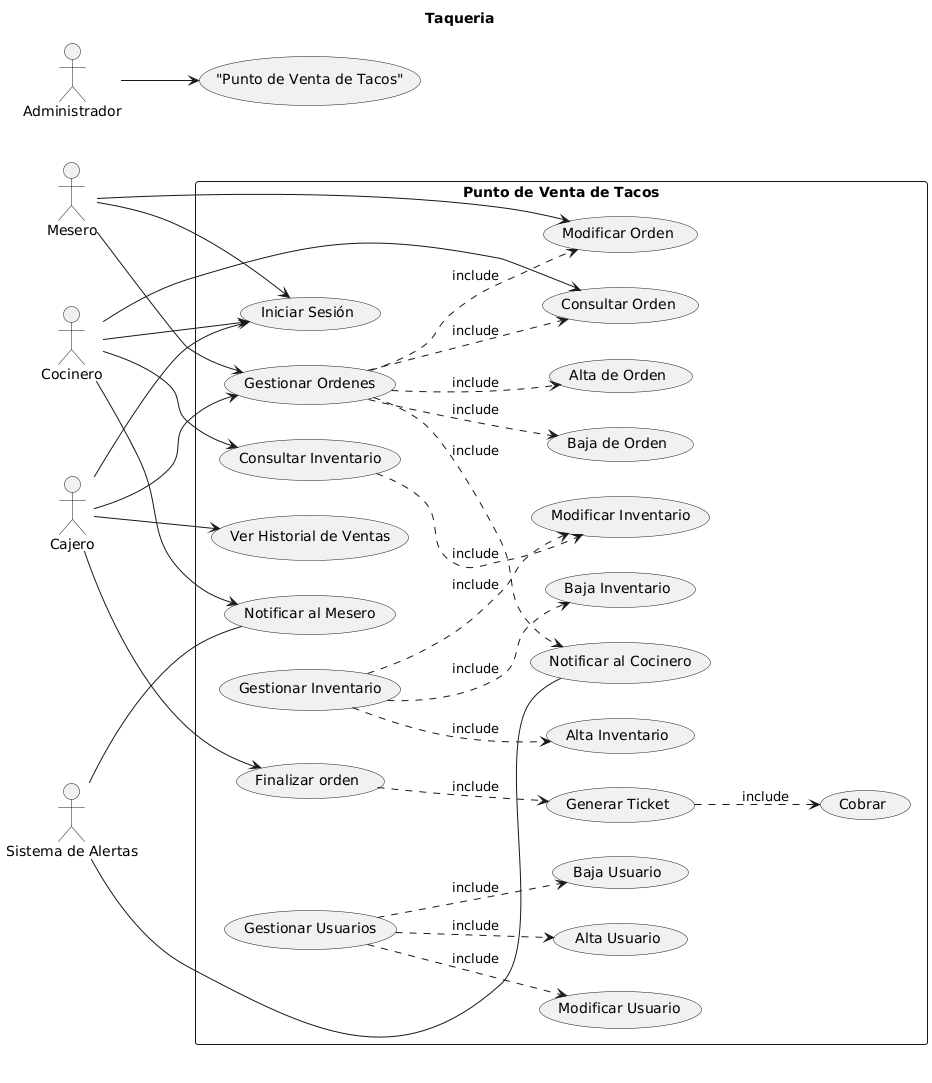
\includegraphics[width=1\textwidth]{casos/uml.png}
    \caption{Diagrama de Casos de Uso del Sistema de Taquería}
    \label{fig:diagrama_casos_uso}
\end{figure}

\subsection{Diagrama Entidad-Relación}
\begin{figure}[H]
    \centering
    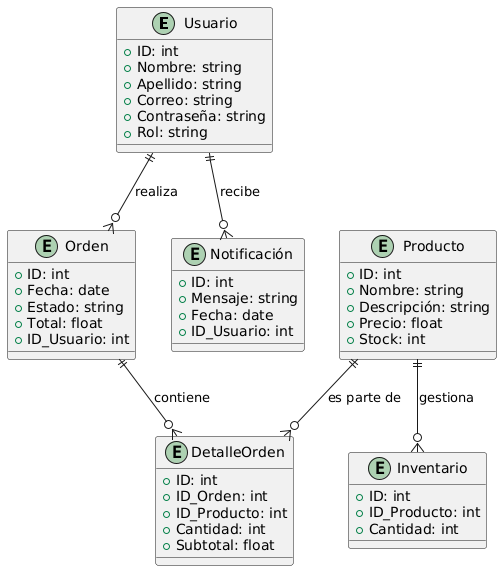
\includegraphics[width=1\textwidth]{casos/EntidadRelacion.png}
    \caption{Diagrama Entidad-Relación del Sistema de Taquería}
    \label{fig:diagrama_er}
\end{figure}

\end{document}
